\documentclass{sig-alternate}

\begin{document}

\title{Ruído Natural na Filtragem Colaborativa}
\subtitle{[Trabalho Final]}

\numberofauthors{3}

\author{
\alignauthor
    Paulo Xavier
    \email{\affaddr{contato.pauloxavier@gmail.com}}
% 2nd. author
\alignauthor
    Gabriel Segobia
    \email{\affaddr{segobia.gos@gmail.com}}
% 3rd. author
\alignauthor
    Fellipe Bravo
    \email{\affaddr{fellipe.bravo@gmail.com}}
}
\additionalauthors{}
\date{22 fevereiro 2017}

\copyrtyr={2017} 
\global\acmcopyr={}

\maketitle

\begin{abstract}
Foi mostrado recentemente que os usuários podem ser inconsistentes quando eles elicitam avaliações para itens, expondo os dados usados nos SR à inconsistências. Esse trabalho busca quantificar o impacto do ruído na predição por modelos, e o desempenho dos algoritmos de detecção de ruído propostos por \emph{O'Mahony} e \emph{Toledo}.
\end{abstract}

\section{Introdução}

Sistemas de Recomendações(SR) são ferramentas de software e técnicas que fornecem sugestões de itens que sejam de uso ao usuário. Existem diversas abordagens que podem ser usadas em SR, e uma das mais populares é a \emph{Collaborative Filtering(CF)}, que produz recomendações específicas a um usuário baseado em padrões de avaliação ou uso de itens.

Em SR é assumido que as avaliações nos \emph{datasets} estão livres de irregularidades. Foi mostrado recentemente que os usuários podem ser inconsistentes quando eles elicitam avaliações para itens, expondo os dados usados nos SR à inconsistências. Esse tipo de inconsistência é conhecida como \emph{ruído natural}. Abordagens que buscam \emph{detectar} e \emph{corrigir} essas avaliações inconsistentes surgiram para resolver esse problema em aberto.

O artigo será organizado da seguinte forma: Seção 3 faz uma revisão de filtragem colaborativa. Seção 4 elicita o problema e faz uma proposta para quantificar o impacto do ruído nos modelos e qual o desempenho dos algoritmos \emph{Mahony} e \emph{Toledo} na detecção de ruído natural. Seção 5 faz uma discussão sobre os experimentos feitos para avaliar o impacto do ruído nos modelos, apresenta os resultados e mostra o \emph{dataset} utilizado para o artigo, além da metodologia usada para obtenção dos resultados obtidos. A seção 5 apresenta uma conclusão sobre os resultados obtidos e propostas para trabalhos futuros sobre o tema.

\section{Filtragem Colaborativa}
\emph{Filtragem Colaborativa} é um algoritmo de recomendação popular que baseia suas predições e
recomendações nas avaliações ou comportamento de outros usuários no sistema. A principal
suposição por trás desse método é que as opiniões de outros uários podem ser selecionadas eagregadas de maneira que é possivel ter uma predição razoável das preferências um usuário alvo.

Intuitivamente, assume-se também, que se os usuários concordam sobre a qualidade ou relevância de alguns itens, então eles também vão provavelmente concordar sobre outros itens.

A grande maioria dos algoritmos de CF usados atualmente, operam inicialmente gerando
predições de preferência usuário e então produzindo as recomendações deles ranqueando os
itens candidatos por preferências previstas.

Os CFs possuem algumas vantagens notáveis:
\begin{itemize}
	\item Não necessitam de informações sobre conteúdo ou usuários. As  \emph{abordagens puras} utilizam apenas as avaliações para fazer a predição;
	\item Consegue avaliar a experiencia, qualidade e ponto de vista de outras pessoas na predição;
	\item Consegue sugerir \emph{serendipitous items} através da análise de pessoas do comportamento de usuários semelhantes
\end{itemize}
Possui também algumas desvantagens, dentre elas:
\begin{itemize}
	\item Baixa acurácia quando possui poucas informações sobre as avaliações dos usuários(\emph{Cold Start});
	\item Ratings são dados explicitamente por usuários, gerando uma base de dados ruidosa por natureza (\emph{ruído natural e/ou ruído malicioso}).
\end{itemize}

\section{Proposta}
Em SR é assumido que as avaliações nos \emph{datasets} estão livres de irregularidades. Foi mostrado recentemente que os usuários podem ser inconsistentes quando eles elicitam avaliações para itens, expondo os dados usados nos SR à inconsistências.

Ruído em SR pode ser classificado em 2 categorias principais:
\begin{enumerate}
	\item \emph{Ruído Malicioso}, associado ao ruído intencionalmente introduzido por um agente externo para influenciar os resultados de um recomendador, e
	\item \emph{Ruído Natural}, involutariamente introduzido por usuários, e que também poderia afetar o resultado da recomendação.
\end{enumerate}
	
O \emph{ruído natural} é inserido sem intenção maliciosa, e, ao contrário do \emph{ruído malicioso}, que já é estudado na literatura há tempos, é um tópico recente.
	
A identificação do \emph{ruído natural} é mais difícil, pois ele tende a aparecer de diversas formas (ao contrário do malicioso, que costuma estar associado à alguns padrões nos perfis dos usuários).
	
Neste artigo serão usados dois algoritmos para quantificação do impacto do ruído no modelo, \emph{O'Mahony} e \emph{Toledo}.

\subsection{O'Mahony}
O algoritmo de \emph{O'Mahony} considera o quão consistente o rating atual para um par usuário-item é em respeito a avaliação prevista que é feita por algum algoritmo de recomendação G.
 
A \emph{consistência} c de uma avaliação $r_{u,v}$ como o Erro Médio Absoluto (MAE) entre a avaliação atual e a prevista:
	$$ c(G,T)_{u,v} = \frac{|{u,v} - p_{u,v}|}{r_{max} - r_{min}} $$

onde $p_{u,v}$ é a avaliação prevista para o par usuário-item ($u,v$) e $r_{min}/r_{max}$ são o mínimo e máximo dos ratings permitidos, respecivamente. Uma avaliação $r_{u,v}$ é considerada como ruído e excluída do processo de recomendação se:
$$ c(G,T)_{u,v} > th $$
onde $th$ é um valor \emph{threshold}.
\subsection{Toledo}
O algoritmo proposto por \emph{Toledo} inicialmente classifica avaliações, usuários e itens, e que cada item também sua própria tendência de receber avaliações. São identificadas e classificadas conforme a figura 1.

\begin{figure}[h]
\centering
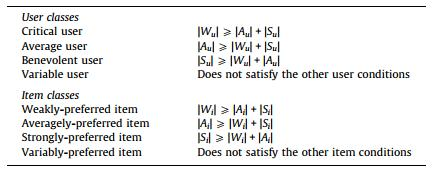
\includegraphics[width=1.0\linewidth]{table_toledo}
\caption{Toledo - Classes de Itens e Usuários}
\label{Figura 1}
\end{figure}


O processo para detecção do ruído assume que para um rating $r(u,i)$ de um dataset, se as classes associadas ao usuário $u$ e o item $i$ pertencem ao meso grupo, então a avaliação deve pertencer a classe de avaliação no mesmo grupo. Se a avaliação não estiver de acordo com a condição, poderia ser uma avaliação ruidosa, e sua transformação poderia mitigar o ruído natural do dataset. Conforme \emph{figura 2}. 

\begin{figure}[h]
\centering
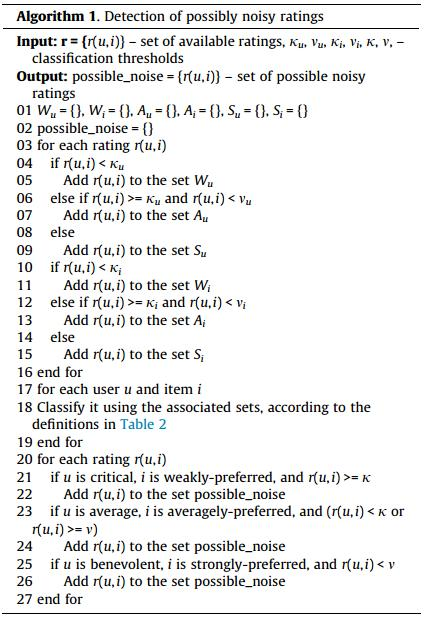
\includegraphics[width=1.0\linewidth]{detec_ruido_toledo}
\caption{Toledo - Detecção de ruído}
\label{Figura 2}
\end{figure}

Após detectar as possíveis avaliações ruidosas a próxima fase lida com essas avaliações, corrigindo a anomalia ao invés de removê-la para evitar perda de informação. Conforme \emph{figura 3}.

\begin{figure}[h!]
	\centering
	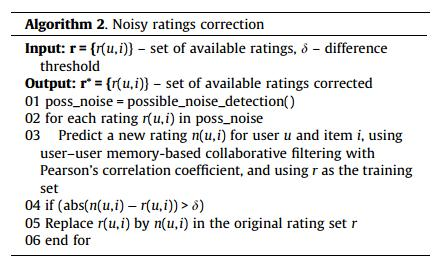
\includegraphics[width=1.0\linewidth]{correcao_toledo}
	\caption{Toledo - Correção de ruído}
	\label{fig:correcao_toledo}
\end{figure}

Conforme literatura, não há disponível nenhum \emph{dataset} que não possua ruído natural, logo para testar a acurácia dos algoritmos não é possível usar um \emph{dataset} totalmente apropriado. Para fins desse artigo, iremos considerar que o \emph{dataset} que utilizamos não possui ruído, e a partir do mesmo iremos inserir ruído malicioso na base e em seguida testar a acurácia dos mesmos usando o \emph{Precision} e \emph{Recall}.


\section{Experimentos}


\subsection{Dataset}
Para este artigo, foi utilizado o dataset fornecido pelo \emph{Movie Lens Research Project}. \emph{MovieLens} é um SR \emph{web-based} de filmes que começou a operar em 1997.

Consiste de 943 usuários, 1682 filmes e contém 100,000 avaliações no total. As avaliações são baseadas numa escala de 1 a 5.

\subsection{Metodologia}

A inserção do ruído será feita aleatoriamente iterando de 1 a 10\% da base e executando os algoritmos de \emph{Toledo} e \emph{O'Mahony} para detectar o número de avaliações que foi marcada como ruído no mesmo. Essa inserção será feita invertendo-se as notas na base, transformando ratings de acordo com a tabela abaixo:

\begin{table}[h!]
	\centering
	\label{my-label}
	\begin{tabular}{|c|c|}
		\hline
		\textbf{Rating} & \textbf{Novo Valor} \\ \hline
		\textit{1}      & 5                   \\ \hline
		\textit{2}      & 4                   \\ \hline
		\textit{3}      & 1                   \\ \hline
		\textit{4}      & 2                   \\ \hline
		\textit{5}      & 1                   \\ \hline
	\end{tabular}
	\caption{Troca de Ratings na Inserção de Ruído}
\end{table}


\subsection{Resultados}

\section{Conclusão e Trabalhos Futuros}

\end{document}
